\section{Methods}
\label{sec:methods}

We collect official telemetry and reconstruct it into four STDB object types
on shared time and map axes: moving teams, dynamic safe/blue zones, spatial
events, and phase intervals. The graph-ready population contains 21,824
competitive matches after excluding tutorial/training sessions and a small
number of degenerate telemetry files. We index reconstructed zone-change
intervals as analysis phases 1--8; cut phases are 1--7.

\begin{figure}[htbp]
\centering
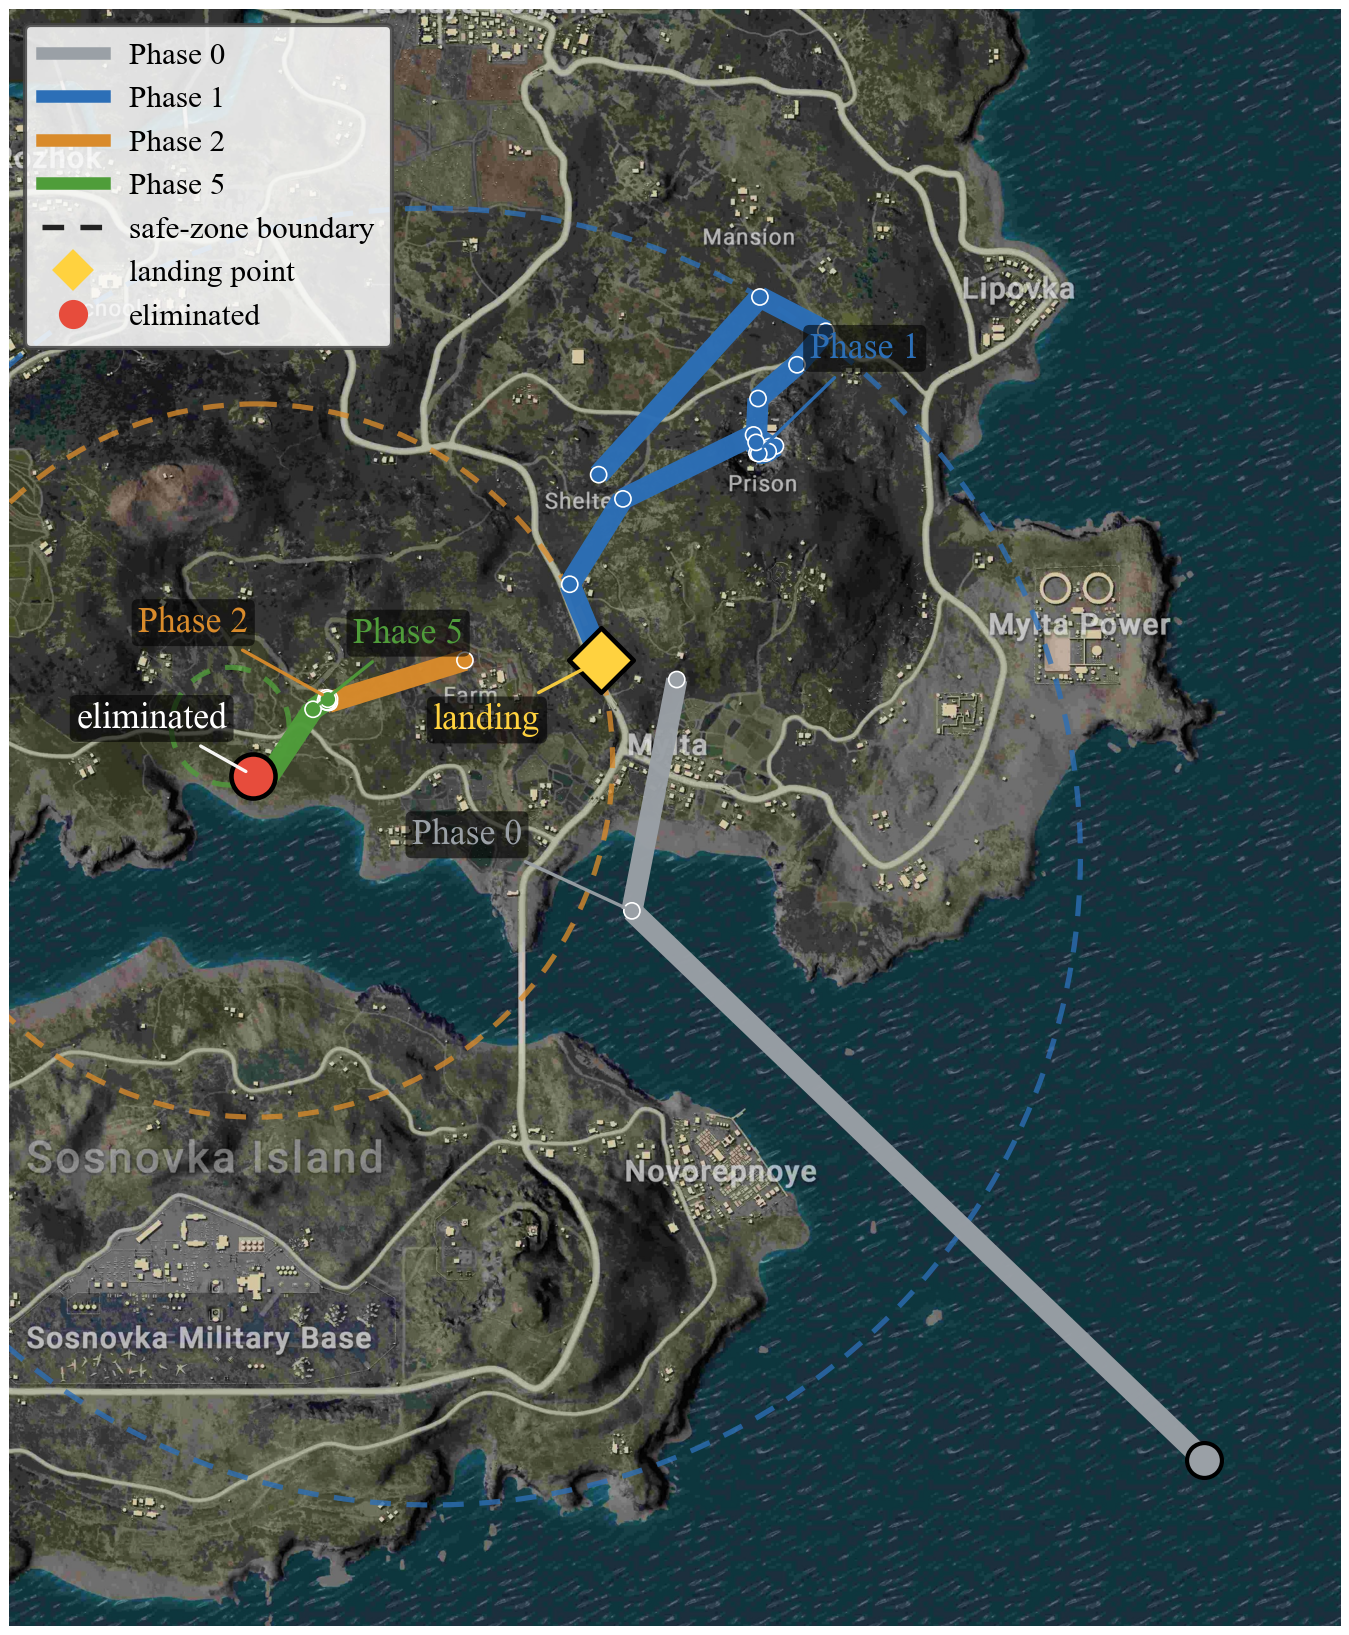
\includegraphics[width=0.96\linewidth]{figures/team_phase_feature_example.png}
\caption{Team-phase STDB example. A team's centroid trajectory is aligned
with phase-specific safe-zone boundaries; the landing point, phase movement,
and elimination point become one phase-indexed spatial history.}
\label{fig:team-phase-feature-example}
\end{figure}

\paragraph{Team-phase features.}
The modeling unit is \((m,i,k)\): match \(m\), team \(i\), phase \(k\).
Each row summarizes one team's phase-local trajectory, zone exposure, combat,
state, and readiness. Table~\ref{tab:feature-sources} separates conventional
telemetry aggregates from the added STDB spatio-temporal features used in the
paper. The \(d\) column is the number of raw tabular variables used in the
representation ablation; DynamicSTGNN uses normalized numeric variants of the
same sources as a 66-dimensional node vector. The STDB-only count includes the
shared phase index, which is counted once in the combined view.

\begin{table}[htbp]
\centering
\caption{Conventional telemetry aggregates and added STDB spatio-temporal
features.}
\label{tab:feature-sources}
\scriptsize
\setlength{\tabcolsep}{2.5pt}
\begin{tabular}{p{0.18\linewidth}p{0.22\linewidth}rp{0.42\linewidth}}
\toprule
Source & Group & \(d\) & Representative features \\
\midrule
Conventional & Match/team state, combat, readiness & 57 &
Phase duration, alive teams/players, health, vehicles, spread, damage,
knockdowns, kills, combat partners, items, healing/boost use \\
Added STDB & Trajectory, zone/enemy exposure & 16 &
Team-centroid path length, displacement, speed, rotation timing, safe-zone
alignment and entry time, boundary distance, outside-zone ratio, enemy density,
nearest-enemy distance \\
Combined view & Conventional+STDB & 72 &
Hazard-prediction input combining conventional aggregates with STDB
trajectory/exposure features \\
\bottomrule
\end{tabular}
\end{table}

Team position is the centroid of surviving members; team spread and
nearest-enemy quantities compensate for split squads. All features are
computed from observations inside the phase and scaled by fixed
feature-specific constants. Variables that can occasionally take very large
values, such as damage, item pickups, and combat-event counts, are
log-compressed. Each DynamicSTGNN team-phase node is represented by the
66-dimensional normalized vector derived from these sources.
Figure~\ref{fig:team-phase-feature-example} shows the spatial view captured
by this row-level representation.

\paragraph{Dynamic team graphs.}
For each phase we define a weighted heterogeneous graph
\(G_k=(V_k,X_k,\{A_k^r\}_{r\in R})\). Nodes are teams, \(X_k\) is the feature
matrix, and \(R\) contains three relations. Proximity is a symmetric
distance-decay edge between team centroids. Combat is directed from attacker
to victim and grows with damage, knockdowns, and kills. Co-pressure links
nearby teams that are jointly outside, or near the boundary of, the safe
zone. All relation weights are computed only from observations inside phase
\(k\). Before graph aggregation, the outgoing weights of each team are scaled
to sum to one, so that a team combines information from its connected
opponents without the magnitude depending only on how many links it has.
The proximity relation also keeps the team's own feature vector in the
aggregation.
Figure~\ref{fig:dynamic-graph-example} illustrates the conversion from a
phase-level STDB snapshot to the graph structure used by the model.

\begin{figure*}[htbp]
\centering
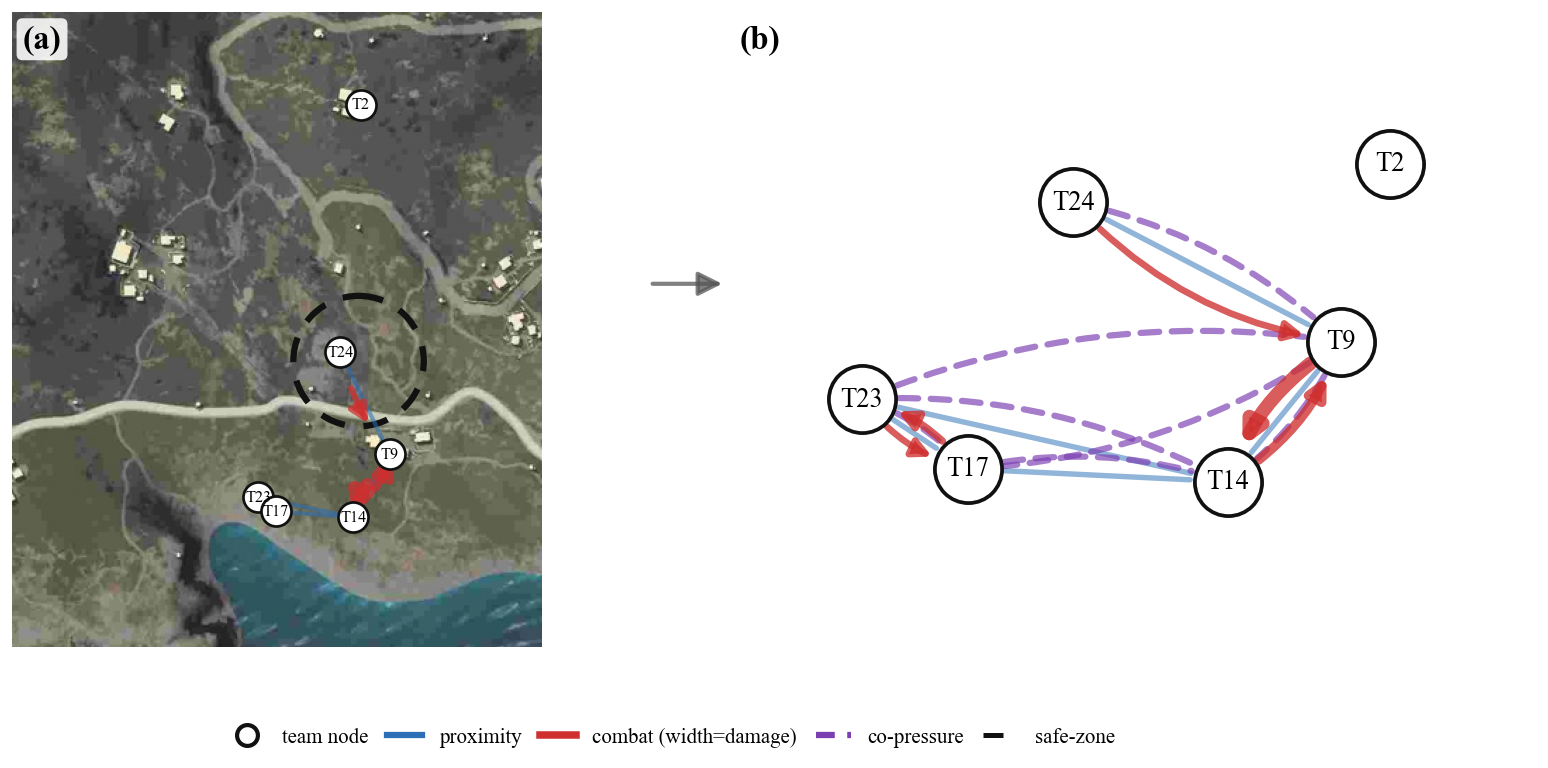
\includegraphics[width=0.86\textwidth]{figures/dynamic_heterogeneous_graph_example.png}
\caption{Dynamic heterogeneous graph example. A phase-level STDB snapshot
with team centroids, the safe-zone boundary, and combat events is converted
into proximity, combat, and co-pressure relations between teams.}
\label{fig:dynamic-graph-example}
\end{figure*}

\paragraph{Hazard task and model.}
At the end of each indexed phase, the risk set contains teams that are still
alive and have an observed next phase. Let \(b_k\) be the end time of phase
\(k\), and \(T_i\) the elimination time of team \(i\). The binary label is
\[
Y_{i,k}=\Ind\!\left\{b_k < T_i \leq b_{k+1}\right\}, \qquad
h_{i,k}=P(Y_{i,k}=1 \mid T_i>b_k, X_{i,\leq k}).
\]
Thus \(Y_{i,k}=1\) means that team \(i\) survives through \(b_k\) but is
eliminated before the next phase ends. Teams already eliminated at \(b_k\),
padded team slots, and cells without an observed next phase are excluded by
the mask.

DynamicSTGNN takes the sequence of team-phase features together with the
sequence of proximity, combat, and co-pressure graphs. It summarizes both
temporal change within each team and relations among teams, then outputs one
hazard score for each cut phase.
